\section{Experiment} \label{sec:experiments}
% move to set up\subsection{Baseline Evaluation}
% We begin our evaluation by establishing a baseline using Empirical Risk Minimization (ERM) without any augmentation or specialized sampling strategies. This baseline serves as a control to illustrate inherent challenges in class-imbalanced scenarios. The resulting model performance highlights significant classification bias toward majority classes, as evidenced by high accuracy in majority classes but notably poor performance in minority classes. These results underscore the necessity of advanced methods capable of mitigating such imbalance-driven biases.

\subsection{Setup}
\textbf{Dataset Overview.}
Our experiments are conducted on five benchmark datasets: SVHN-10~\cite{netzer2011reading}, CIFAR-10~\cite{krizhevsky2009learning}, CINIC-10~\cite{darlow2018cinic}, CIFAR-100~\cite{krizhevsky2009learning}, and TinyImageNet-200~\cite{le2015tiny}. Following the methodology in \cite{cao2019learning}, we generate synthetically imbalanced versions of each dataset to evaluate model performance under these conditions. To ensure statistical robustness, all results are reported as the mean and standard deviation over three independent runs.

\begin{figure*}[htb]
    \centering
    \begin{subfigure}[b]{0.30\textwidth}
        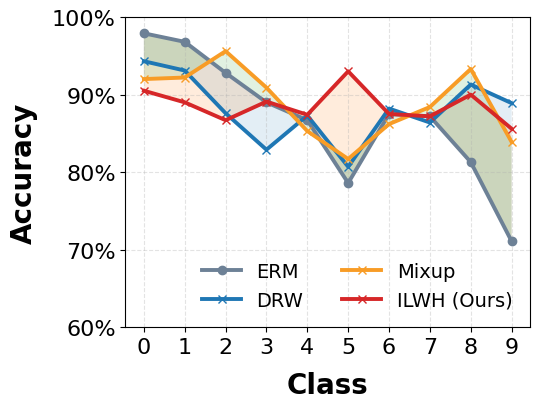
\includegraphics[width=\textwidth]{cinic_auto.png}
        \caption{Auto-aug -- CINIC-10}
        % \vspace{-7pt}
        \label{fig:cinic_auto}
    \end{subfigure}
    \begin{subfigure}[b]{0.30\textwidth}
        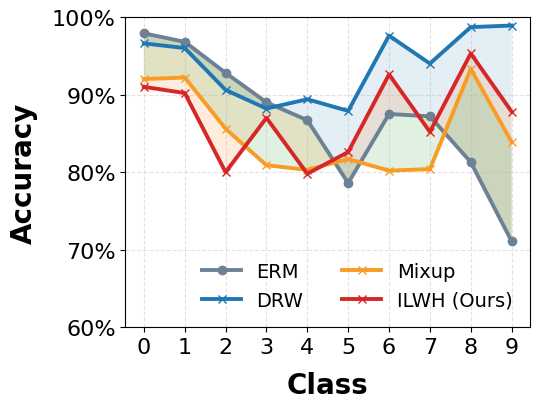
\includegraphics[width=\textwidth]{cinic_cutout.png}
        \caption{Cutout -- CINIC-10}
        % \vspace{-7pt}
        \label{fig:cinic_cutout}
    \end{subfigure}
    \begin{subfigure}[b]{0.30\textwidth}
        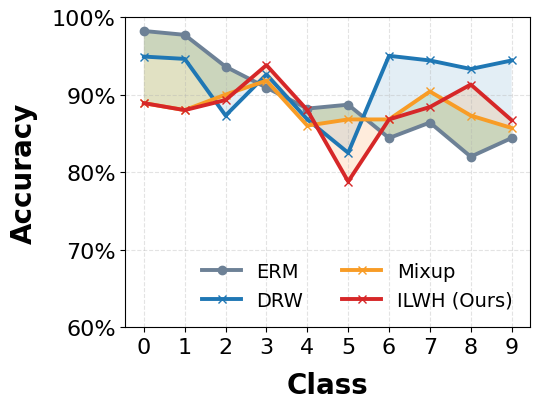
\includegraphics[width=\textwidth]{cinic10_rand.png}
        \caption{Rand-aug -- CINIC-10}
        % \vspace{-7pt}
        \label{fig:cinic10_rand}
    \end{subfigure}
    \begin{subfigure}[b]{0.30\textwidth}
        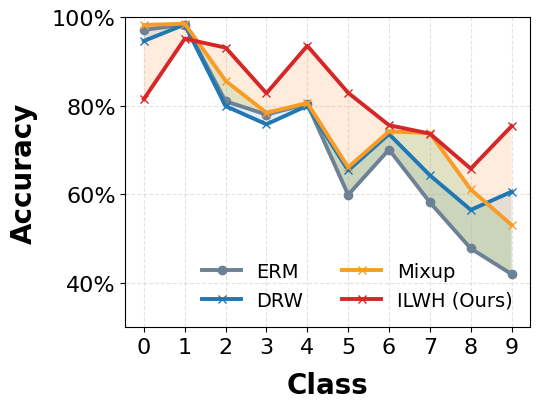
\includegraphics[width=\textwidth]{cifar10_auto.png}
        \caption{Auto-aug -- CIFAR-10}
        % \vspace{-7pt}
        \label{fig:cifar10_auto}
    \end{subfigure}
    \begin{subfigure}[b]{0.30\textwidth}
        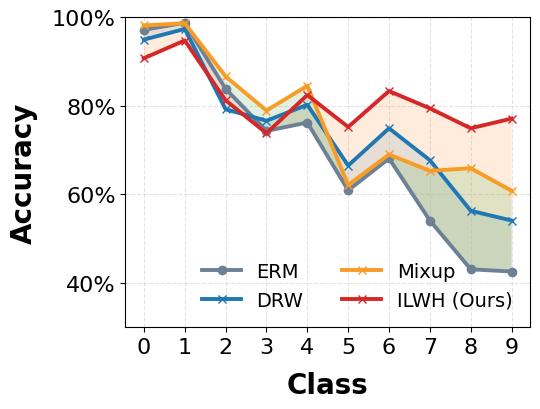
\includegraphics[width=\textwidth]{cifar10_cutout.png}
        \caption{Cutout -- CIFAR-10}
        % \vspace{-7pt}
        \label{fig:cifar10_cutout}
    \end{subfigure}
    \begin{subfigure}[b]{0.30\textwidth}
        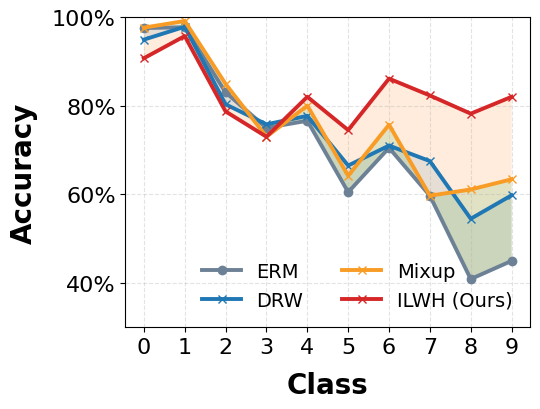
\includegraphics[width=\textwidth]{cifar10_randaug.png}
        \caption{Rand-aug -- CIFAR-10}
        % \vspace{-7pt}
        \label{fig:cifar10_randaug}
    \end{subfigure}
        \begin{subfigure}[b]{0.30\textwidth}
        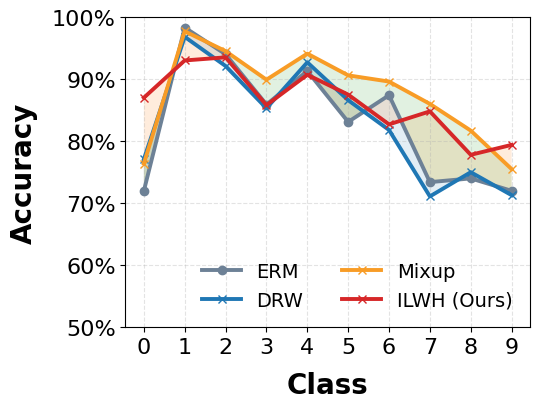
\includegraphics[width=\textwidth]{svhn_auto.png}
        \caption{Auto-aug -- SVHN-10}
        % \vspace{-7pt}
        \label{fig:svhn_auto}
    \end{subfigure}
    \begin{subfigure}[b]{0.30\textwidth}
        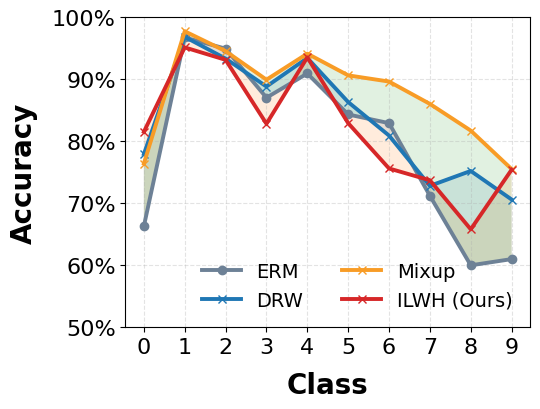
\includegraphics[width=\textwidth]{svhn_cutout.png}
        \caption{Cutout -- SVHN-10}
        % \vspace{-7pt}
        \label{fig:svhn_cutout}
    \end{subfigure}
    \begin{subfigure}[b]{0.30\textwidth}
        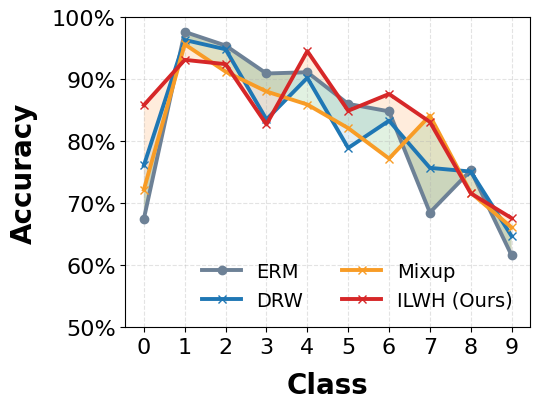
\includegraphics[width=\textwidth]{svhn_randaug.png}
        \caption{Rand-aug -- SVHN-10}
        % \vspace{-7pt}
        \label{fig:svhn_randaug}
    \end{subfigure}
    \caption{Comparison of per-class accuracy across different strategies, affected by different data augmentation methods. Proposed methods (\textit{DRW, Mixup, and ILWH}) consistently outperform ERM, with particularly large gains observed in minority (\textit{tail}) classes. This demonstrates that such sampling strategies not only improve overall accuracy but also enhance learning in underrepresented classes, addressing class imbalance more effectively.}
\end{figure*}

\textbf{Introducing Class Imbalance.} To evaluate our methods under imbalanced conditions, we artificially create long-tail imbalanced versions of the datasets. This was done consistently for all datasets using a fixed imbalance factor of 0.01. The process involves programmatically reducing the number of training samples per class according to the target exponential distribution. Specifically, for each class, we randomly selected a predetermined number of instances from the original dataset, discarding the remainder. For example, after this transformation, the training sample counts for the 10 classes in CIFAR-10 were set to \texttt{[5000, 2997, 1796, 1077, 645, 387, 232, 139, 83, 50]}, creating a controlled imbalanced environment for our experiments.
\begin{table*}[htb]
\centering
\caption{Computational complexity and training efficiency on CIFAR-10.}
\label{tab:complexity_cifar10}
\renewcommand{\arraystretch}{1.2}
\setlength{\tabcolsep}{1.2pt}
\begin{tabular}{lccccc}
\hline
 \textbf{Method} &\textbf{IwT} & \textbf{Avg FLOPs/Epo (G)} & \textbf{Total FLOPs (G)} & \textbf{Avg Time/Epo (s)} & \textbf{Rel. Cost} \\
\hline
M2m & \cmark & 6{,}589.37 & 1{,}317{,}873.27 & 6.32 & 1.00$\times$ \\
DeepSMOTE & \xmark & $\approx$9{,}884--13{,}179 & $\approx$1.98--2.64$\times 10^{6}$ & $\approx$9.5--12.6 & $\approx$1.5--2.0$\times$ \\
ILWH (Ours) & \cmark & 6{,}589.37 & 1{,}317{,}873.27 & \textbf{5.03} & \textbf{0.80$\times$} \\
\hline
\end{tabular}
\begin{tablenotes}
    \item \textit{\textbf{Integrate within Training (IwT)}}: \textit{The data augmentation process is generated within training progress. DeepSMOTE generates synthetic data before starting the training progress.}
\end{tablenotes}
\end{table*}

\textbf{Classification model.}
All methods use an identical ResNet-32 \cite{he2016deep} as their base classifier.

\textbf{Configuration.}
The training process involved the baseline data augmentation, where each image was padded by 4 pixels on each side, followed by a random 32 × 32 crop from the padded image or its horizontally flipped version. The model was trained for 200 except for TinyImageNet-200 in which it was trained for 300 epochs. The learning rate was initially set to 0.1 and decayed by a factor of 0.01. Additionally, a linear warm-up strategy was applied for the first 5 epochs to stabilize training and ensure a fair comparison~\cite{goyal2017accurate}. 

\textbf{Training Mode.}
The experiments were carried out using four training strategies: using ERM as a loss function, DRW, Mixup and our proposed ILWH.

\textbf{Performance Metrics.}
Performance is measured through metrics such as group accuracy for many-shot, medium-shot, and low-shot classes, confusion matrix-derived class recall, \textit{precision@1} and \textit{precision@5} for top predictions, and average loss tracking.

\subsection{Data Augmentation Experiment}
In our experimental evaluation, specific settings were adopted for each of the data augmentation techniques to ensure reproducibility and align with common practices.

For \textit{AutoAugment}, we employed the predefined and appropriate policies learned for each specific dataset to guide the augmentation. For CIFAR-10, CIFAR-100, and CINIC-10, we used the \texttt{AutoAugmentPolicy.CIFAR10}. This single policy is suitable for all three as they share similar image characteristics and content domains. For the SVHN-10 dataset, we applied its specifically trained \texttt{AutoAugmentPolicy.SVHN}. Similarly, for experiments involving Tiny-ImageNet-200, we utilized the \texttt{AutoAugmentPolicy.ImageNet}, which was originally discovered on the full ImageNet dataset. This approach ensures that the augmentation strategies are well-suited to the underlying distribution of each dataset.
\begin{figure*}[htb]
    \centering
    \begin{subfigure}[b]{1.0\textwidth}
        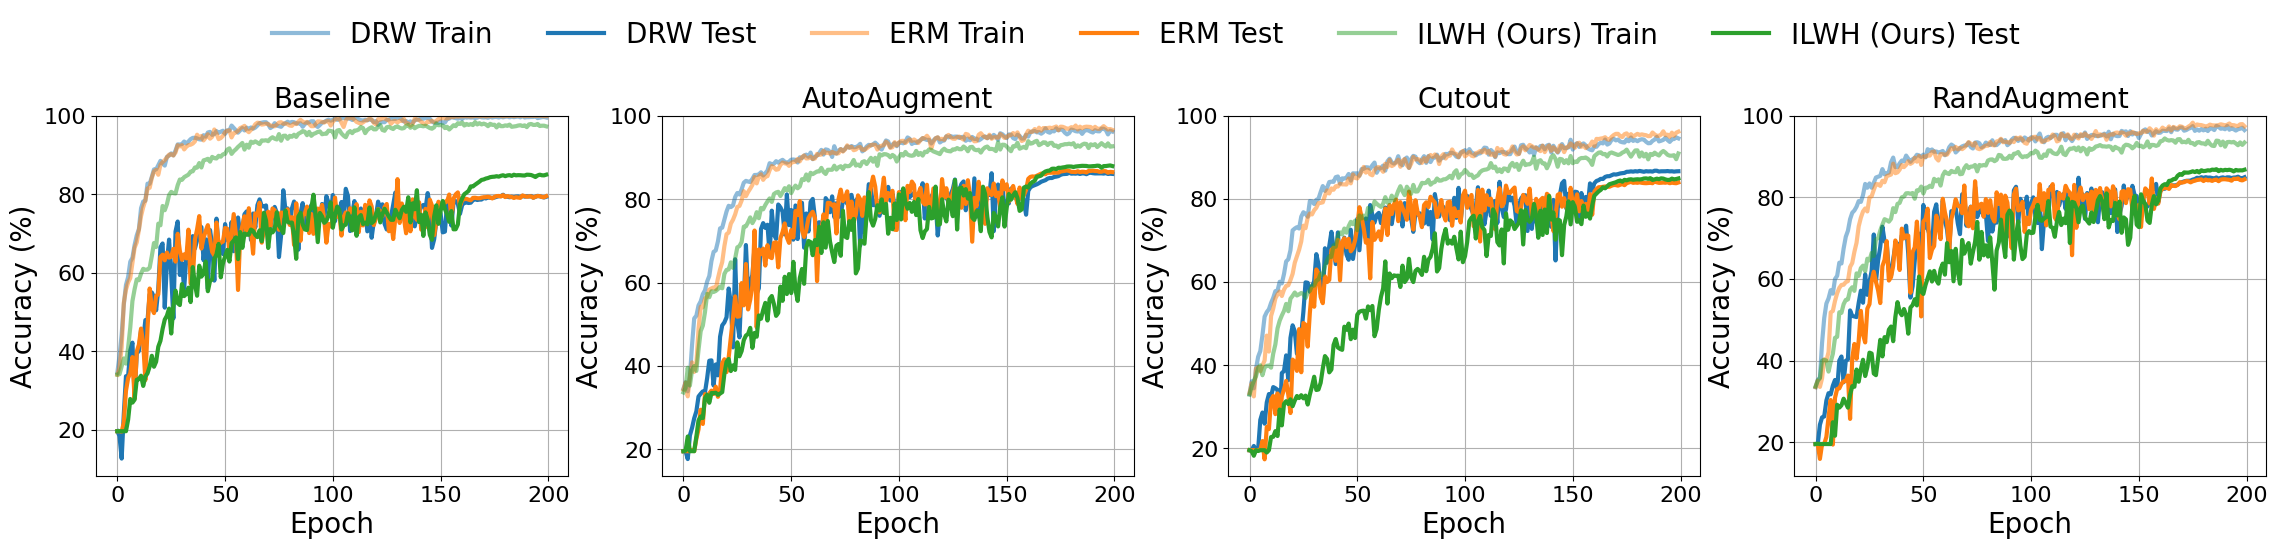
\includegraphics[width=\textwidth]{svhn_exp.png}
        % \caption{SVHN}
        \vspace{-5pt}
        \label{fig:svhn_exp}
    \end{subfigure}
    \begin{subfigure}[b]{1.0\textwidth}
        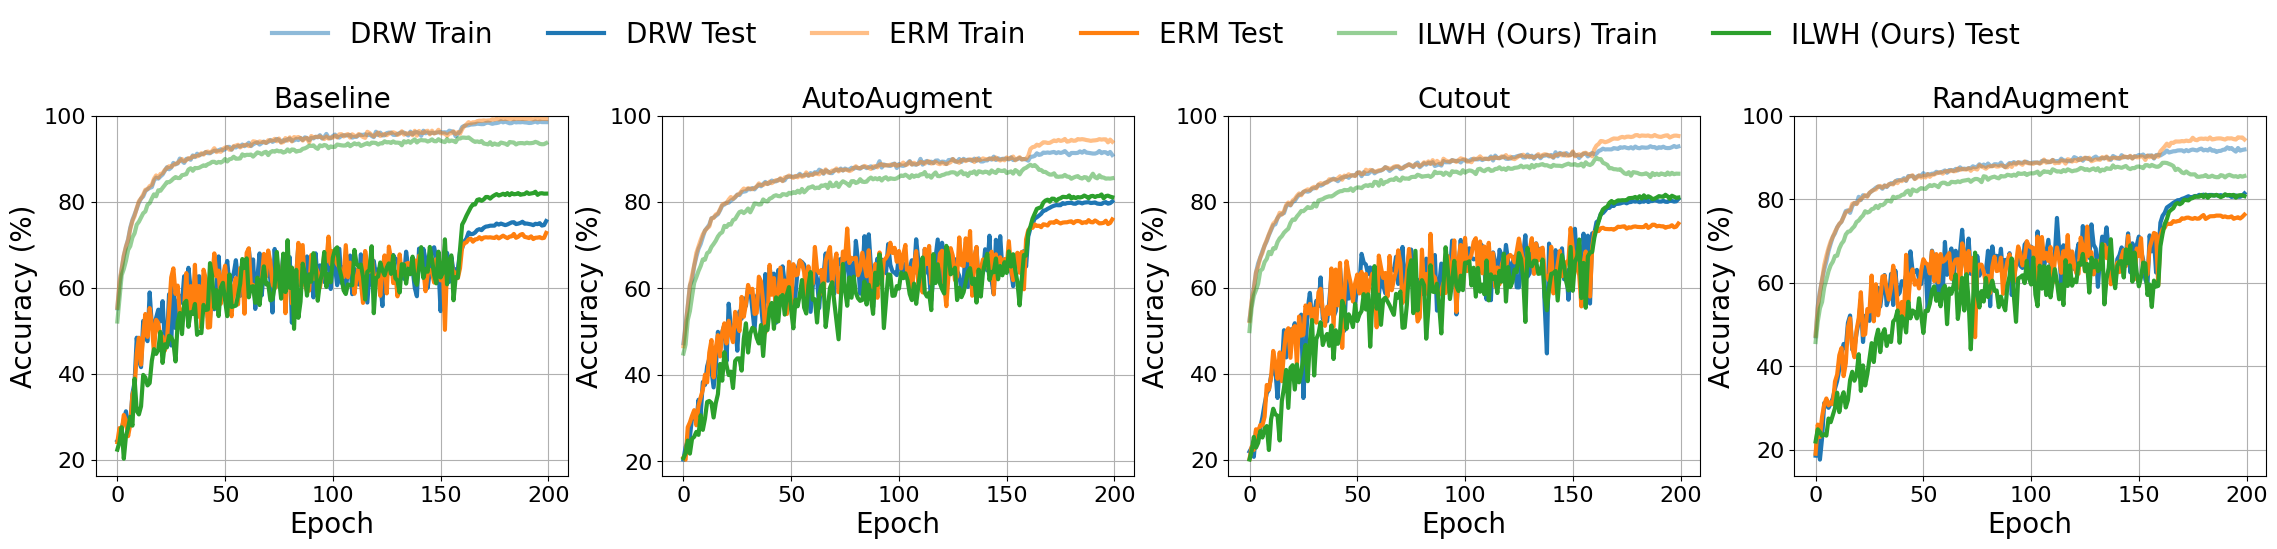
\includegraphics[width=\textwidth]{cifar10_exp.png}
        % \caption{CIFAR-10}
        \vspace{-5pt}
        \label{fig:cifar10_exp}
    \end{subfigure}
    \begin{subfigure}[b]{1.0\textwidth}
        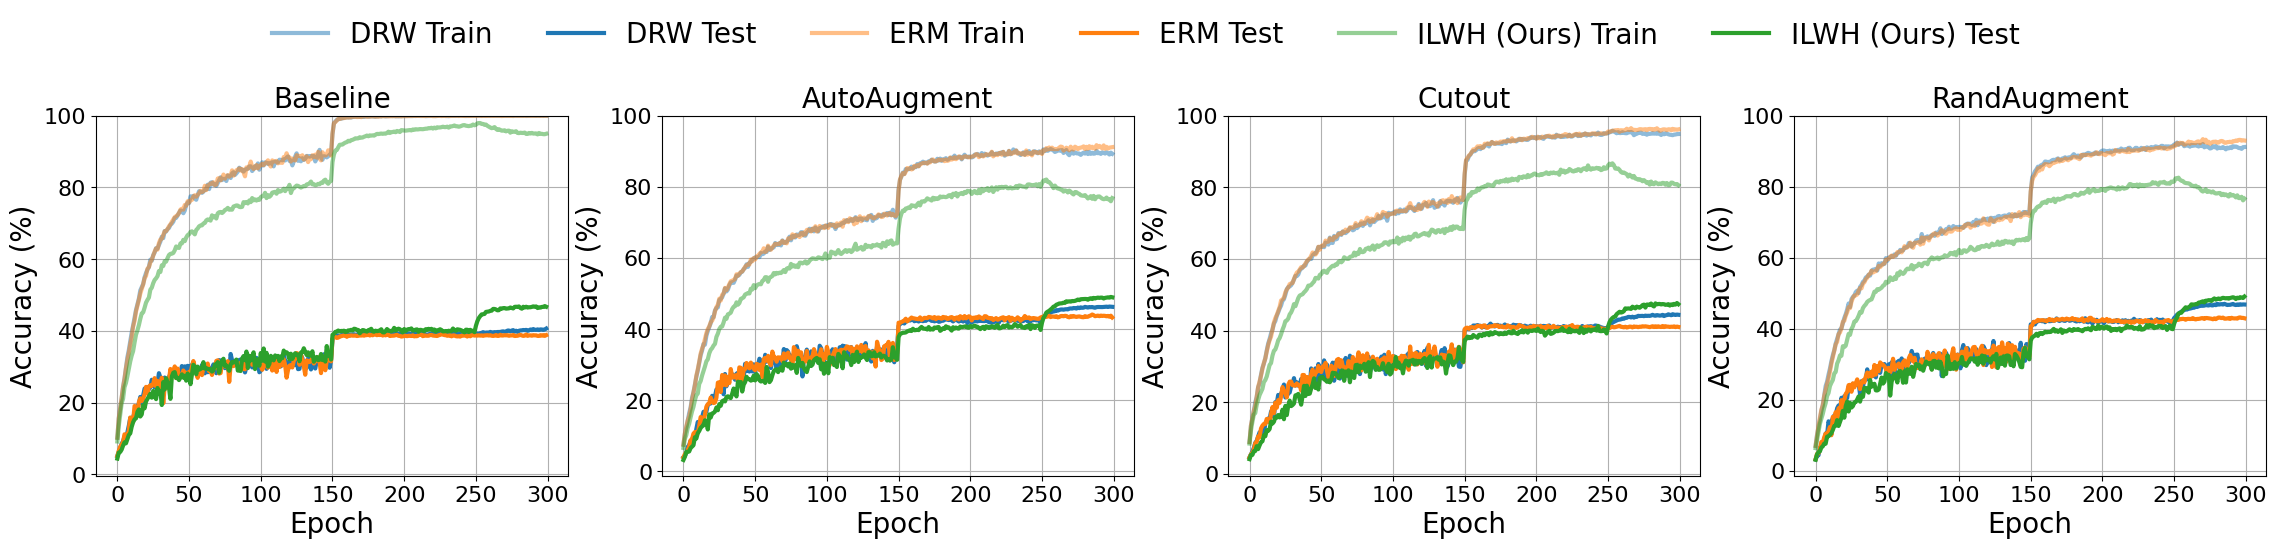
\includegraphics[width=\textwidth]{cifar100_exp.png}
        % \caption{CIFAR-100}
        \vspace{-5pt}
        \label{fig:cifar100_exp}
    \end{subfigure}
    \caption{Training and testing accuracy curves on SVHN-10 (\textbf{top}), CIFAR-10 (\textbf{middle}) and CIFAR-100 (\textbf{bottom}) with different data augmentation methods.}
\end{figure*}

Regarding \textit{RandAugment}, which offers a simplified approach to automated augmentation, we set its two primary hyperparameters as follows: the number of augmentation transformations to apply sequentially, $N$, was chosen as 2, and the global magnitude for these transformations, $M$, was set to 14. These values were selected based on common settings that balance augmentation strength and computational efficiency.

For the \textit{Cutout} regularization technique, our experiments involved applying a randomly positioned square mask of size $16 \times 16$ pixels to the input images during training. This size was chosen to introduce a moderate level of occlusion, encouraging the model to learn more distributed features.

\subsection{Data Sampling Experiment}

For our main comparative experiments, we fixed this parameter to \(\alpha=0.5\) across all datasets to maintain a consistent and moderate level of balancing. It is important to note that this sampling process occurs after the data augmentation transformation. These sampling strategies were integrated directly into the training pipeline by passing a custom batch sampler to the \texttt{DataLoader}. This ensures that each mini-batch is constructed according to the specified sampling logic, rather than simple sequential or random sampling over the entire dataset.

\subsection{Computational Efficiency Analysis}

We evaluated the computational complexity of each method using the ptflops package and measured wall-clock training time. As shown in Table \ref{tab:complexity_cifar10}, \textbf{ILWH (Ours)} requires FLOPs identical to the M2m baseline (6.59 × 10³ G per epoch) but reduces average epoch time by approximately 20\% . In contrast, \textbf{DeepSMOTE} introduces substantially higher computational overhead ($\sim$1.5--2$\times$) due to its encoder-decoder generation module, which increases both forward- and backward-pass costs. This analysis confirms that the proposed \textbf{ILWH (Ours)} design maintains computational efficiency while improving performance on imbalanced data, while generative oversampling approaches like DeepSMOTE trade efficiency for synthetic diversity \cite{dablain2022deepsmote}.

\subsection{Result Analysis}
According  to the results in  Table \ref{tab:drw_results_cifar_svhn_cinic} and Table \ref{tab:drw_results_cifar100_tiny}, the overall performance of  ILWH achieved effectiveness across different  datasets when compared to introduced methods. To be precise in Table  \ref{tab:drw_results_cifar_svhn_cinic}, our methodology has outperformed the other ones with \textbf{top 1 Accuracy} when conducted on common augmentations and several samplings. It is a strong  evidence that our research potentially can optimize not only computing-resources but also overall model performances. Despite these promising results on datasets with less complex patterns and smaller sample sizes (\textit{e.g., CIFAR-10, SVHN-10, CINIC-10}), the performance on the more challenging CIFAR-100 and TinyImageNet-200 datasets remains at a tolerable level. Post-training accuracies for these complex tasks generally range from 30\% to nearly 50\%. Nevertheless, as reflected in the aforementioned tables, our research not only introduces an innovative approach to address this ingrained problem but also offers a promising direction for future AI researchers to achieve higher performance without the need for intensive computational resources.

The experimental results presented in Figures \ref{fig:drw_affect}, \ref{fig:comparision_m2m_deepSMOTE_Ours}, and \ref{fig:weight_dist} collectively demonstrate the effectiveness of the proposed lightweight imbalanced learning method. As shown in Figure \ref{fig:drw_affect}, applying the DRW strategy after the $160^{th}$ epoch leads to a significant reduction in both training and testing losses. Before applying DRW, the model experiences a slower decline in loss, indicating that it is learning general features without being overly influenced by class imbalance. However, once DRW is introduced, the loss curves drop sharply, suggesting that the model benefits from the delayed application of class weight. This delayed balancing allows the model to first learn stable representations and then focus on minority classes later in training, thereby improving convergence stability and generalization performance.

Figure \ref{fig:comparision_m2m_deepSMOTE_Ours} further supports these findings by comparing the proposed method with other resource-intensive techniques such as M2m and DeepSMOTE on the CIFAR-10 and CIFAR-100 datasets. On CIFAR-10, the proposed approach achieves comparable accuracy to these heavy models while maintaining computational efficiency. Similarly, on CIFAR-100, it delivers competitive results, demonstrating that the combination of lightweight augmentations and DRW can achieve high accuracy without requiring complex architectures or extensive computational resources. This result confirms the strength of the proposed method in achieving a balance between efficiency and performance.

In Figure \ref{fig:weight_dist}, the normalized class weight distribution across training epochs provides insight into how DRW dynamically adjusts learning focus. At the beginning of training, the weight is almost uniform across classes, indicating that the model treats all samples equally. After DRW is activated at epoch $160^{th}$, the weight of minority classes gradually increases while those of majority classes remain stable or slightly decrease. This adaptive re-weighting ensures that underrepresented classes receive more attention in the later training stages, helping to mitigate class imbalance and improve recognition of rare categories.